\chapter{Spatial enhancement methods}

\section{Problem statement}

Implement the image enhancement task of Section 3.7 (Fig 3.43) (Section 3.8, Fig 3.46 in our slides).\\
The image to be enhanced is \textit{skeleton\_orig.tif}.\\
You should implement all steps in Figure 3.43. \\
(You cannot directly use functions of Matlab such as
imfilter or fspecial, implement all functions by yourself).

\section{Python implementation}

Usage:~\textbf{python problem2.py [-h] [--laplacian] [--sobel] [-a A] image\_path} \\

For example, to use a 3x3 Laplacian filter with A = 1.7, and then a Sobel, type:~\\

\textbf{python problem2.py --laplacian -a 1.7 --sobel skeleton\_orig.tif} \\

The original image, its Laplacian, its sharpened (Laplacian) and its Sobel will be displayed.

\pagebreak
\section{Results}

    \subsection{Original image}

    \begin{figure}[!htb]\centering
        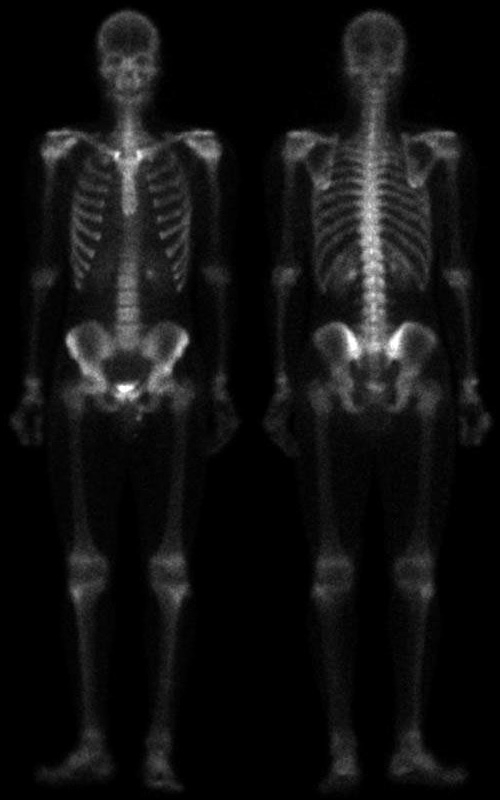
\includegraphics[width=0.7\linewidth]{./images/2/skeleton.jpg}
        \caption{Original \textit{skeleton\_orig.tif}}
        \label{diagram:skeleton}
    \end{figure}


    \pagebreak
    \subsection{3x3 Laplacian (A = 0)}

    \begin{figure}[!htb]\centering
        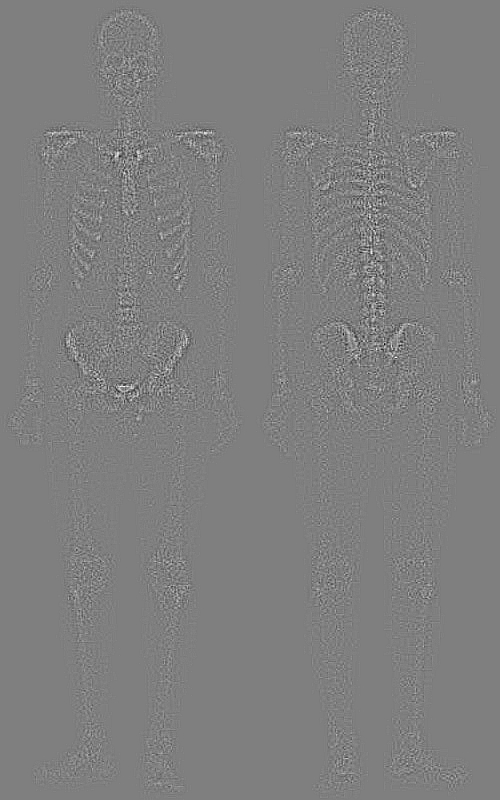
\includegraphics[width=0.4\linewidth]{./images/2/laplacian_A0.jpg}
        \caption{Laplacian (A=0)}\label{diagram:laplacian_0}
    \end{figure}

    \begin{figure}[!htb]\centering
        \begin{minipage}{0.40\textwidth}
            \frame{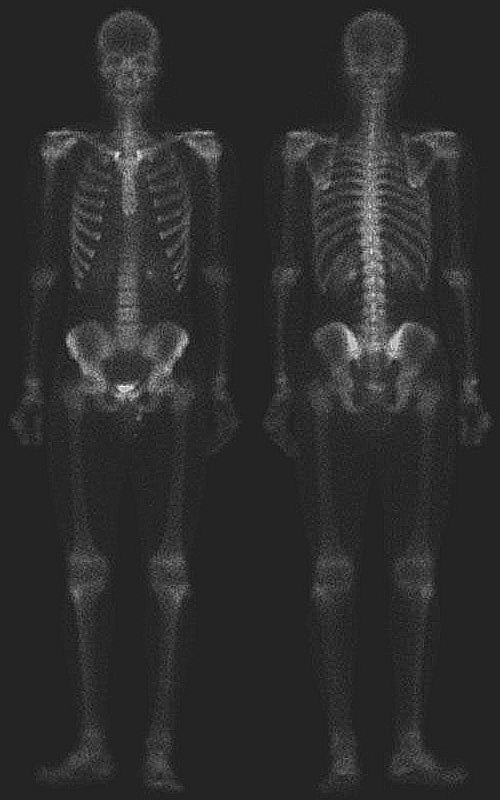
\includegraphics[width=\linewidth]{./images/2/laplacian_A0_sharpened.jpg}}
            \caption{Sharpened image}\label{diagram:laplacian_0_sharpened}
        \end{minipage}
        \begin{minipage}{0.40\textwidth}
        \frame{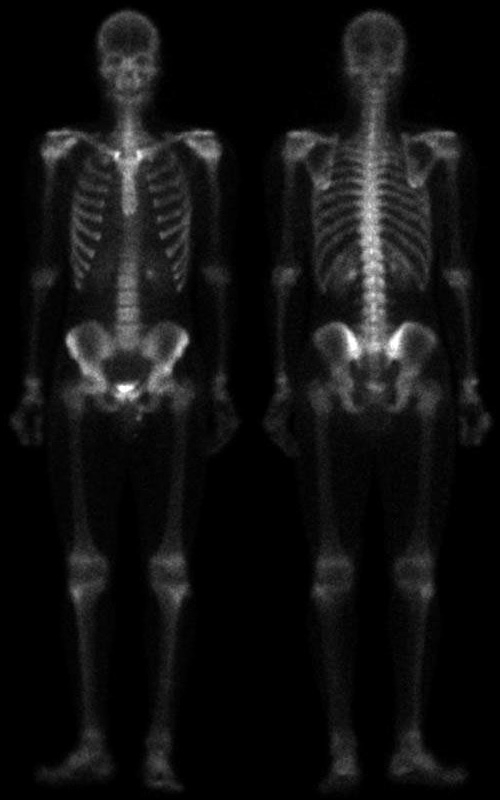
\includegraphics[width=\linewidth]{./images/2/skeleton.jpg}}
        \caption{Original image}
        \end{minipage}
    \end{figure}


    \pagebreak
    \subsection{3x3 Laplacian (A = 1)}

    \begin{figure}[!htb]\centering
        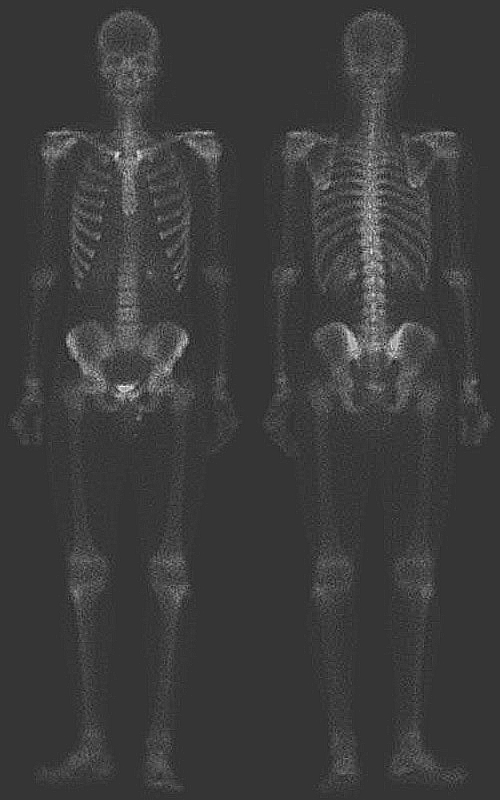
\includegraphics[width=0.4\linewidth]{./images/2/laplacian_A1.jpg}
        \caption{Laplacian (A=1)}\label{diagram:laplacian_1}
    \end{figure}

    \begin{figure}[!htb]\centering
        \begin{minipage}{0.40\textwidth}
            \frame{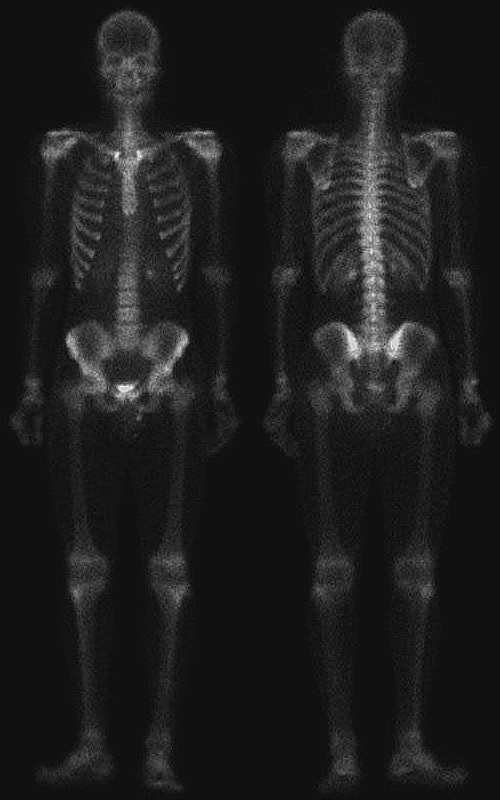
\includegraphics[width=\linewidth]{./images/2/laplacian_A1_sharpened.jpg}}
            \caption{Sharpened image}\label{diagram:laplacian_1_sharpened}
        \end{minipage}
        \begin{minipage}{0.40\textwidth}
        \frame{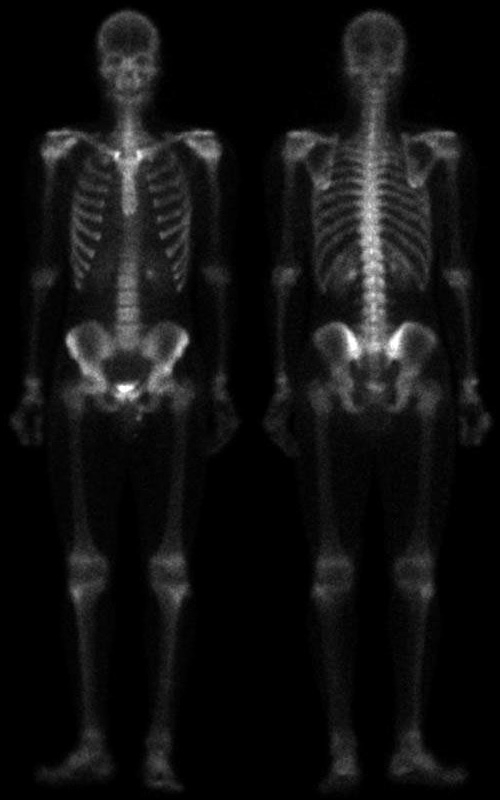
\includegraphics[width=\linewidth]{./images/2/skeleton.jpg}}
        \caption{Original image}
        \end{minipage}
    \end{figure}


    \pagebreak
    \subsection{3x3 Laplacian (A = 1.7)}

    \begin{figure}[!htb]\centering
        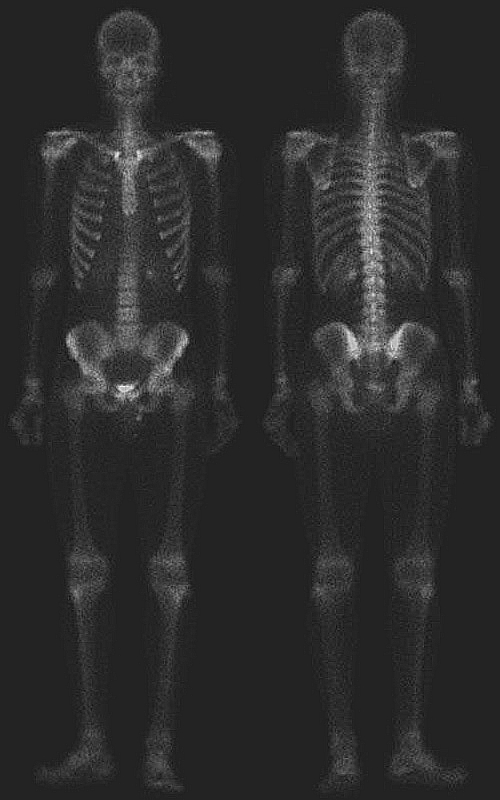
\includegraphics[width=0.4\linewidth]{./images/2/laplacian_A1-7.jpg}
        \caption{Laplacian (A=1.7)}\label{diagram:laplacian_1_7}
    \end{figure}

    \begin{figure}[!htb]\centering
        \begin{minipage}{0.40\textwidth}
            \frame{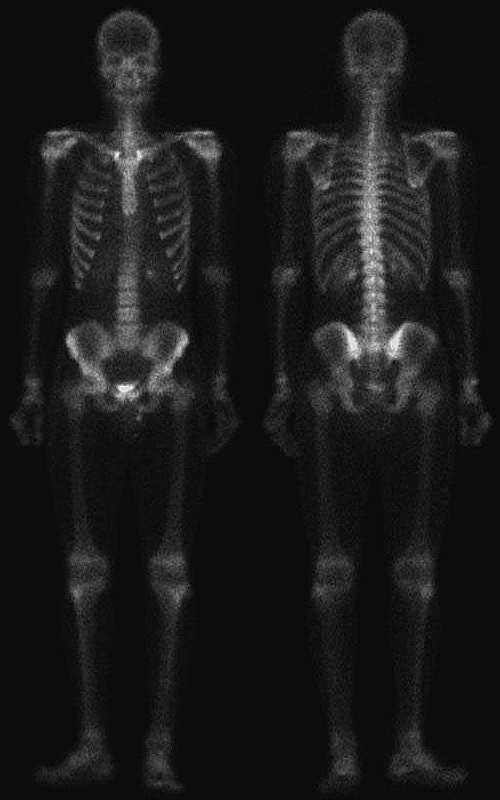
\includegraphics[width=\linewidth]{./images/2/laplacian_A1-7_sharpened.jpg}}
            \caption{Sharpened image}\label{diagram:laplacian_1_7_sharpened}
        \end{minipage}
        \begin{minipage}{0.40\textwidth}
        \frame{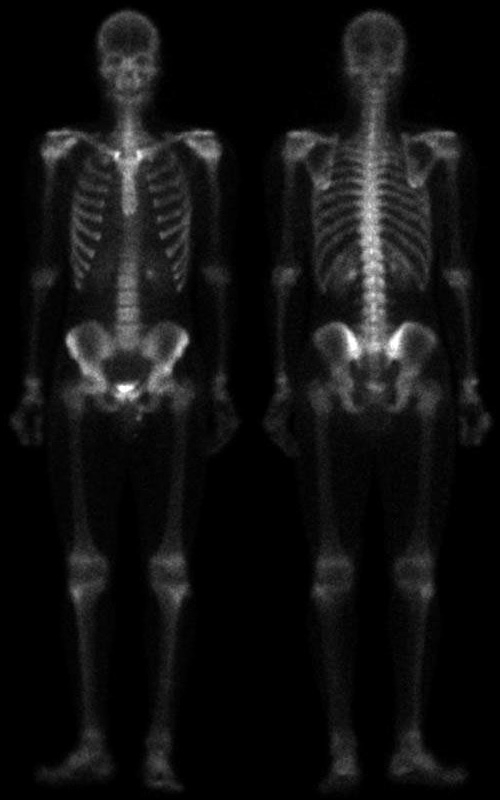
\includegraphics[width=\linewidth]{./images/2/skeleton.jpg}}
        \caption{Original image}
        \end{minipage}
    \end{figure}


    \pagebreak
    \subsection{Sobel}

    \begin{figure}[!htb]\centering
        \begin{minipage}{0.40\textwidth}
            \frame{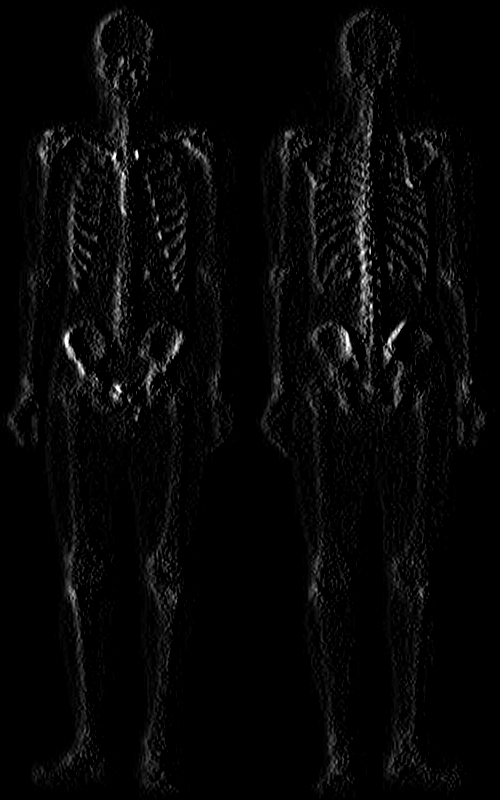
\includegraphics[width=\linewidth]{./images/2/sobel_x_gradient.jpg}}
            \caption{Sobel x-gradient}\label{diagram:sobel_x_gradient}
        \end{minipage}
        \begin{minipage}{0.40\textwidth}
        \frame{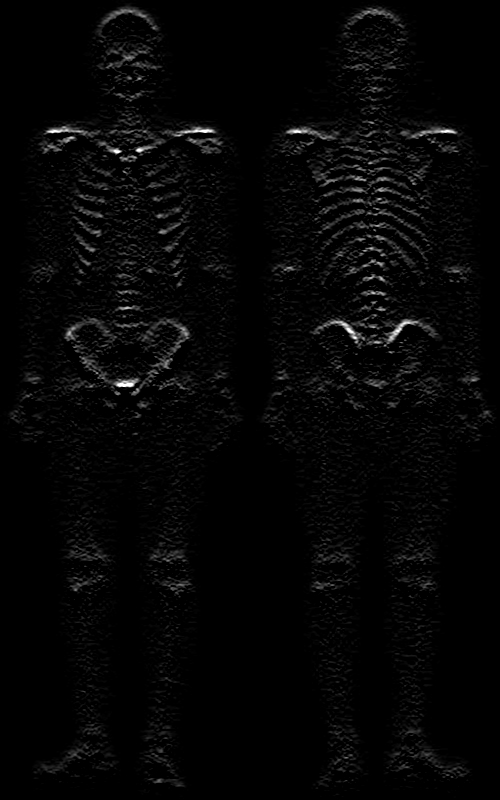
\includegraphics[width=\linewidth]{./images/2/sobel_y_gradient.jpg}}
        \caption{Sobel y-gradient}\label{diagram:sobel_y_gradient}
        \end{minipage}
    \end{figure}

    \begin{figure}[!htb]\centering
        \begin{minipage}{0.40\textwidth}
            \frame{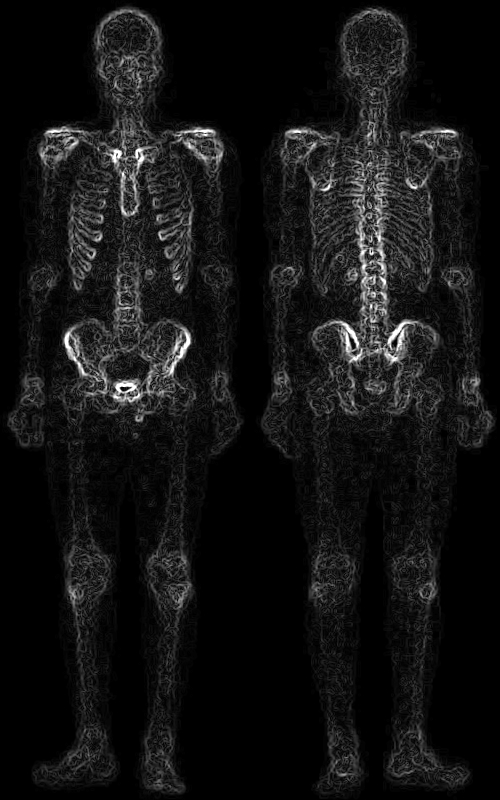
\includegraphics[width=\linewidth]{./images/2/sobel.jpg}}
            \caption{Sobel image}\label{diagram:sobel}
        \end{minipage}
        \begin{minipage}{0.40\textwidth}
        \frame{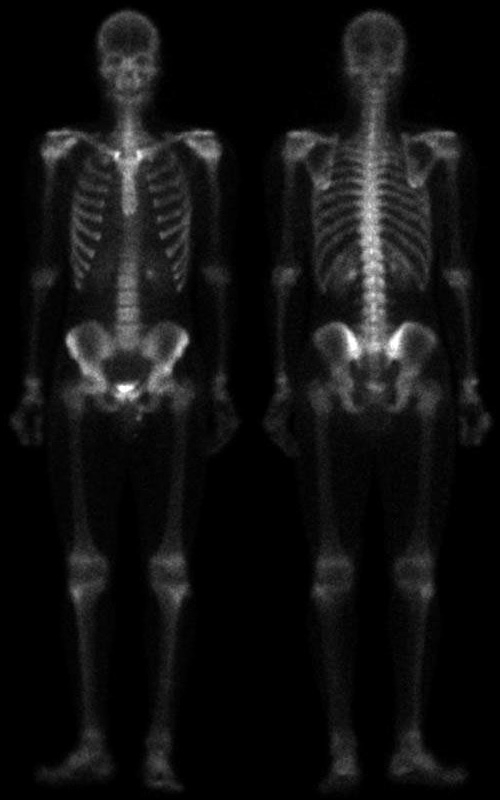
\includegraphics[width=\linewidth]{./images/2/skeleton.jpg}}
        \caption{Original image}
        \end{minipage}
    \end{figure}
